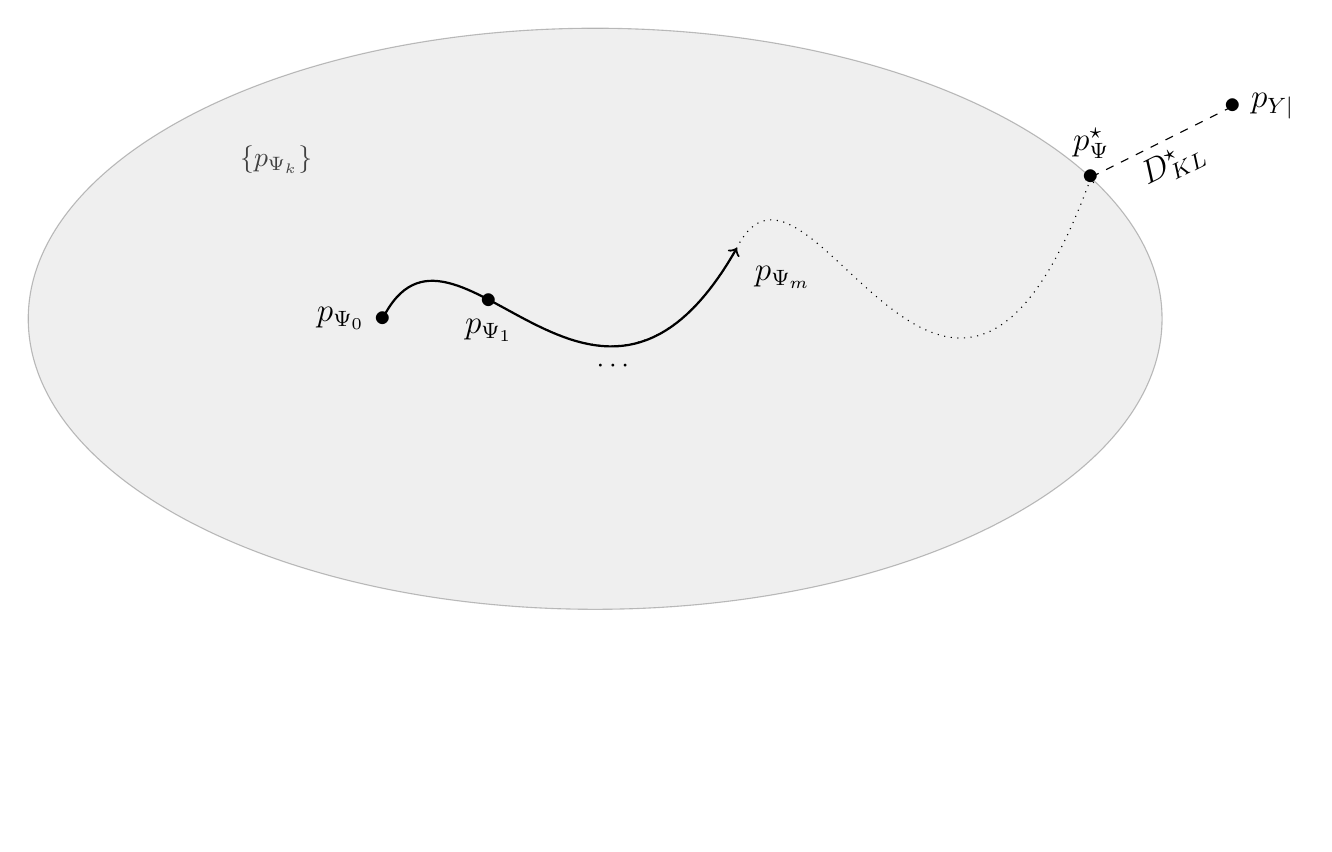
\begin{tikzpicture}[scale = 0.9]
    \draw[fill = lightgray, opacity = 0.25] (3,0) ellipse (8cm and 4.1cm);
    \coordinate (P0) at (-1,0);
    \coordinate (P1) at (0,0);
    \coordinate (P2) at (1,2);
    \coordinate (P3) at (3,-2.5);
    \coordinate (P4) at (5,1);
    \coordinate (P5) at (6,3);
    \coordinate (P6) at (8,-3.5);
    \coordinate (P7) at (10,2);
    \coordinate (P8) at (11,4);
    \coordinate (P9) at (12,-2);
    \coordinate (P10) at (15,0);
    
    \draw[->,thick] (P1) .. controls (P2) and (P3) ..
          (P4);
    
    \draw[dotted,->] (P1) .. controls (P2) and (P3) ..
          (P4) .. controls (P5) and (P6) ..
          (P7);
    
    \draw (0,0)     node{\large$\bullet$}node[left = 3pt]{\large $p_{\Psi_0}$};
    \draw (1.5,0.25)  node{\large$\bullet$}node[below = 3pt]{\large $p_{\Psi_1}$};
    \draw (3.25,-0.45) node[below]{$\cdots$};
    \draw (5,1)     node[below right= 3pt]{\large $p_{\Psi_m}$};
    \draw (10,2)    node{\large$\bullet$}node[above = 3pt]{\large $p_{\Psi}^\star$};
    \draw (-1.5,2.25)    node[color = gray!50!black]{$\{p_{\Psi_k}\}$};
    
    \draw (12,3) node{\large$\bullet$}node[above, right = 3pt]
    	{\large $p_{Y|\Xhat}$};
    \draw[dashed] (10,2) -- (12,3) node[midway,below,sloped]
    	{\large $\text{D}_{\text{KL}}^\star$};
    \draw (0,-7) node{};
\end{tikzpicture}
